
\documentclass[12pt]{article}
\usepackage[a4paper,width=150mm,top=25mm,bottom=25mm]{geometry}
\usepackage{graphicx}
\usepackage{array}
\usepackage{tikz}
\usepackage{wrapfig}
\usepackage{subcaption}
\usepackage[export]{adjustbox}
\usepackage{lipsum}
\usepackage{fontspec}
\usepackage{textcomp,gensymb}
\graphicspath{{./images/}}
\usepackage{amsmath,amssymb,amsthm}
\usepackage{ragged2e}
\usepackage{minted2}
\usepackage{verbatim}

%compile with latexmk -lualatex -shell-escape main.tex

\numberwithin{figure}{section}

\begin{document}
\begin{titlepage}
  \begin{center}
  \begin{tabular}{ m{3cm} m{8cm} m{3cm} }
    \hspace*{-1cm}
\includegraphics[height=0.22\textwidth]{Unigrb} &
 \justifying \textbf{\large UNIVERZITET U NIŠU\newline ELEKTRONSKI FAKULTET} &
    \raggedleft 
\includegraphics[width=0.17\textwidth]{elfak} \\ 
  \end{tabular}
\end{center}

  \vspace{4cm}
\begin{center}
 \begin{tabular}{ m{8cm} m{4cm} m{2cm} }
  \centering\textbf{\large Izveštaj iz predmeta Projektovanje elektronskih sistema}\\
\end{tabular}
\end{center}
\begin{center}
 \begin{tabular}{ m{8cm} m{5cm} m{2cm} }
  \centering\textbf{\Huge Sistem za automatsko zalivanje bašta}\\
\end{tabular}
\end{center}
\vfill 
\begin{tabular}{m{6cm} m{8cm} m{6cm}}
  \raggedright\textsc{\small Studenti:} \\
  \textsc{\small Marko Popović 19323} \\ 
  \textsc{\small Petar Ristić 18881} &
\raggedleft\textsc{\small Profesor:} \\
\raggedleft\textsc{\small  Prof. dr Borisav Jovanović } \\
  \raggedleft \textsc{\small } 
\end{tabular}
\end{titlepage}
\newpage
\tableofcontents
\newpage

\section{Opis zadatkta}
Projektovati sistem za automatizovano zalivanje biljaka u baštama.
Sistem sadrži sledeće funkcionalne celine: uređaje za zalivanje sa pumpom (do 16 Slejv uređaja) koji se instaliraju u baštama; jedan Master automat i centralni računarski sistem. 
Slejv uređaji su preko RS-232 povezani sa Master automatom koji prikuplja informacije sa Slejv uređaja. 
Master automat je dalje povezan preko ETHERNET veze sa centralnim računarom.

Uređaj za zalivanje sa pumpom omogućava zalivanje biljaka po unapred definisanom programu rada. 
Zalivanje se odvija tako što u definisanom vremenskom trenutku početka zalivanja uređaj uključuje pumpu, a isključuje je posle određenog vremena. 
Vremena uključivanja pumpe i vremensko trajanje zalivanja definisani su programom rada. 
Postoji 16 različitih programa rada koji se zadaju sa centralnog računara.
Pošto se smatra da je baštu dovoljno zalivati jednom dnevno, u svakom programu definisano je po jedno vreme uključivanja pumpe, vreme trajanja zalivanja (u sekundama).
Uređaj za zalivanje poseduje taster za manuelno pokretanje/zaustavljanje procesa zalivanja.
Kada se zalivanje pokrene manuelno, isključuje se ili manuelno ili automatski posle isteklog vremena trajanja zalivanja definisanog u tekućem programu rada.
Manuelno zaustavljanje moguće je i kada zalivanje otpočne automatski. 
Protok vode kroz pumpu prati se očitavanjem senzora protoka. 
Ukoliko je protok izvan unapred zadatog opsega (minimalni i maksimalni protok) aktivira se zvučni alarm.
Uređaj za zalivanje poseduje LCD na kome se prikazuju osnovni podaci o tekućem programu rada, statusu sistema, tekućem vremenu.
Ukoliko je započeto zalivanje na LCD-u se prikazuje i koliko vremena je preostalo do isključivanja pumpe.

Centralni računar treba da omogući:
\begin{itemize}
  \item{Očitavanje statusa uređaja za zalivanje (uključen/isključen, start/stop zalivanja, alarm...) svake sekunde.}
  \item{Definisanje svih 16 programa rada ili definisanje pojedinih vremenskih parametara (vreme uključivanja, trajanje zalivanja) za dati program rada}
  \item{Daljinsko podešavanje maksimalnog i minimalnog dozvoljenog protoka vode kroz pumpu}
  \item{Indikaciju alarma.}
  \item{Manuelno daljinsko uključivanje i isključivanje sistema, kao i daljinsko pokretanje i zaustavljanje procesa zalivanja}
\end{itemize}
\newpage
\section{Funkcionalna i nefunkcionalna specifikacija}
\textbf{Funkcionalna specifikacija :}
  \begin{itemize}
  \item{Sistem se sastoji iz jednog Master i do 16 Slejv automata}
  \item{Master automat predstavlja centralni automat koji prikuplja informacije od svih Slejv automata i upravlja njima}
  \item{Master automatom se upravlja putem Centralnog Računarskog Sistema, a samim tim i Slejv automatima}
  \item{Slejv automati su kontroleri zalivanja koji se nalaze na svakoj bašti i upravljaju protokom i trajanju programa}
  \item{Master automat čuva statusne informacije od svih prisutnih Slejvova}
 \item{Master vrši kalibraciju Sata Realnog Vremena svih Slejv automata na zahtev CRS-a}
 \item{CRS ima funkciju prikazivanja statusa bašte, podešavanja Sata Realnog Vremena i programiranje programa rada}
  \item{Master automat čuva podatke o 16 programa zalivanja, koje dodeljuje Slejvovima na zahtev CRS-a}
  \item{Slejv automat odgovara periodično o svom trenutnom stanju}
  \item{Vrši se prikaz osnovnih podataka na Master ekranu}
\end{itemize}
\textbf{Nefunkcionalna specifikacija :}
\begin{itemize}
  \item{Uređaji moraju biti otporni na vlagu, vodu i prašinu, biti dobro izolovani, zbog svog rada u izloženim sredinama}
  \item{Takođe moraju imati malu potrošnju, i visoku pouzdanost}
\end{itemize}
\newpage
\section{Arhitektura sistema}
  Arhitekturu sistema čine tri osnovne komponente sistema: 
  \begin{itemize}
    \item{Centralni Računarski Sistem (CRS)}
    \item{Master Automat}
    \item{Slave automat}
  \end{itemize}

  \textbf{CRS} je sistem koji služi za upravljanje Master automatom i samim tim i Slejv automatima.
  Povezan je sa Masterom automatom putem Ethernet veze, statičkom IP adresom, na njihovoj lokalnoj mreži. 
  Pristup Master automatu vrši se putem HTTP protokola, kucanjem statičke adrese direknto u browser. \newline

 \textbf{Master automat} upravlja Slejv automatima, kojih ima maksimalno 16.
 Vrši se prozivka svakog Slejva na 125ms, pri kojoj se prikupljaju osnovni podaci o statusu svakog Slejva po protokolu koji će kasnije biti opisan.
 Automati su u slučaju krakte udaljenosti međusobno povezani putem RS-232 protokola, dok je u suprotnom korišćen RS-232 protokol.\newline

 \textbf{Slejv automat} se nalazi kod pumpe svake bašte u sistemu, i upravlja protokom i vremenom operacije pumpe po prethodno definisanom programu koji mu je Master automat dodelio.
 Takođe ima funkciju alarma u slučaju prevelikog ili premalog protoka vode kroz sistem za zalivanje. \newline
 \begin{figure}[hb]
 \centering
 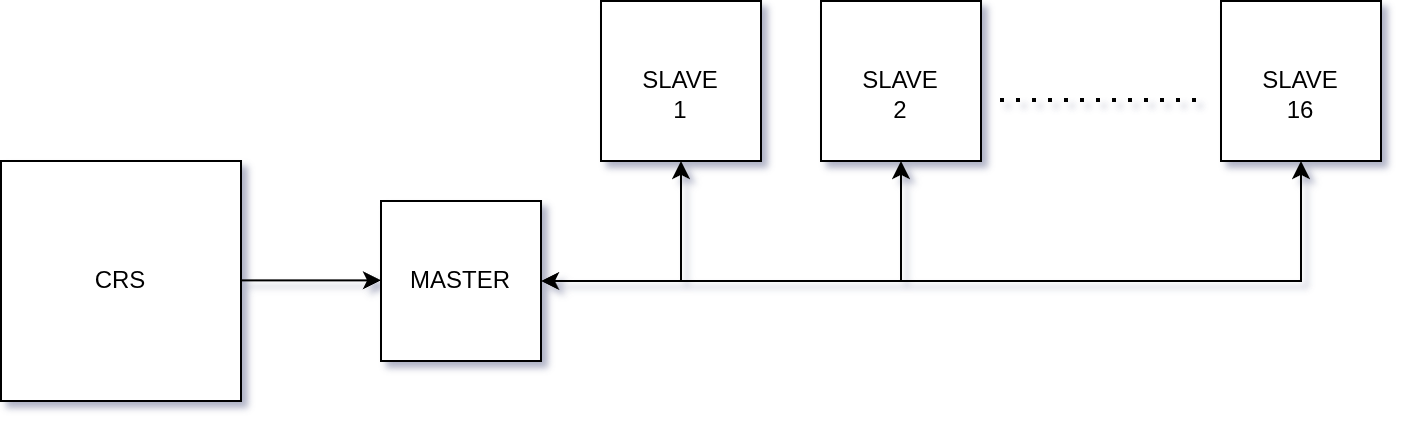
\includegraphics[height=0.25\textwidth]{arch}
 \caption{Dijagram arhitekture sistema}
\end{figure}

  CRS ima jednosmernu komunikaciju ka Masteru, dok Master i Slejv atuomati realizuju obostranu.
\newpage 
\section{Realizacija komunikacionog protokola}

  \subsection{Komunikacija između Master i Slejv automata}

Komunikacija između Master i Slejv automata realizovana je preko UART modula mikrokontrolera i RS-232 drajvera. 
  RS485 je izabran zato što omogućava rad više uređaja na istoj magistrali i pouzdan diferencijalni prenos na većim rastojanjima. 
  U realizovanom sistemu komunikacija radi na bitskoj brzini od 19200 bps, a smer rada RS485 drajvera određuje signal \texttt{DR}. 
  Kada automat šalje podatke, \texttt{DR} se postavlja na logičku jedinicu, a nakon slanja se vraća na nulu da bi automat ponovo slušao magistralu.

  Master periodično proziva Slejv automate. 
  Svaki Slejv ima jedinstveni identifikacioni broj od 0 do 15, koji se u firmveru Slejva čita sa donja četiri bita porta D:
  \[
    \texttt{GARDEN\_ID} = \texttt{PORTD} \& 0x0F
  \]
  Na taj način jedna ista verzija programa može da se koristi na svim Slejv uređajima, a adresa uređaja se podešava prekidačima na razvojnoj ploči.

  U implementiranom protokolu koriste se tri osnovna tipa poruka:
  \begin{itemize}
    \item{\textbf{Prozivka statusa} -- Master šalje jedan bajt oblika \texttt{0x20 | ID}. Slejv čiji se ID poklapa sa donja četiri bita poruke postavlja \texttt{CallFlag} i vraća odgovor od dva bajta.}
    \item{\textbf{Podešavanje sata realnog vremena} -- Master šalje broadcast bajt \texttt{0x7F}, zatim tri bajta: sat, minut i sekund. Slejv primljene decimalne vrednosti konvertuje u BCD cifre koje koristi za interni sat.}
    \item{\textbf{Podešavanje programa zalivanja} -- Master šalje bajt \texttt{0xA0 | ID}, zatim vreme početka programa i trajanje zalivanja. Slejv čuva primljene vrednosti i koristi ih pri automatskom startovanju pumpe.}
  \end{itemize}

  Odgovor Slejv automata na prozivku ili uspešno podešavanje sastoji se iz komandnog bajta i statusnog bajta. 
  Komandni bajt ima oblik \texttt{0x20 | GARDEN\_ID}, čime Master može da proveri od kog Slejva je stigao odgovor. 
  Statusni bajt koristi gornju polovinu bajta za najvažnija stanja uređaja:

  \begin{center}
  \begin{tabular}{|c|c|m{8cm}|}
    \hline
    Bit & Maska & Značenje \\ \hline
    7 & \texttt{0x80} & Sistem je uključen \\ \hline
    6 & \texttt{0x40} & Zalivanje je aktivno \\ \hline
    5 & \texttt{0x20} & Alarm protoka je aktivan \\ \hline
    4 & \texttt{0x10} & Zalivanje je pokrenuto manuelno \\ \hline
  \end{tabular}
  \end{center}

  Preostala četiri bita statusnog bajta ostavljena su slobodna za eventualno proširenje protokola.
  Statusni bajt formira funkcija \texttt{buildStatusByte()}. 
  Ona na osnovu internih promenljivih za uključen sistem, zalivanje, alarm i manuelni režim postavlja odgovarajuće maske.

  Poruka za podešavanje programa zalivanja u realizovanom firmveru sadrži četiri korisna bajta:
  \begin{center}
  \small
  \begin{tabular}{|m{2.4cm}|m{4.5cm}|m{6cm}|}
    \hline
    Redni broj bajta & Promenljiva u Slejvu & Značenje \\ \hline
    1 & \texttt{Tmp\_ProgStartHour} & Sat početka zalivanja \\ \hline
    2 & \texttt{Tmp\_ProgStartMin} & Minut početka zalivanja \\ \hline
    3 & \texttt{Tmp\_time\_left\_high} & Viši deo trajanja zalivanja \\ \hline
    4 & \texttt{Tmp\_time\_left\_low} & Niži deo trajanja zalivanja \\ \hline
  \end{tabular}
  \end{center}
  \normalsize

  Kada se prijem ove poruke završi, postavlja se \texttt{ProgramSetupFlag}. 
  Glavna petlja zatim prebacuje privremene vrednosti u aktivne promenljive programa. 
  Vreme početka se konvertuje u BCD format, jer se u istom formatu vodi interni sat, dok se trajanje zalivanja računa kao:
  \[
    \texttt{WateringSec} = \texttt{time\_left\_high} \cdot 100 + \texttt{time\_left\_low}
  \]
  Time se omogućava da Master pošalje program rada, a Slejv da ga izvršava lokalno bez stalnog nadzora centralnog računara.



  \subsection{Komunikacija između Master automata i Centralnog Računarskog sistema}
    Komunikacija se odvija putem Ethernet porta, kroz web browser na Centralnom Računarskom Sistemu. 
    Master automat podešen je da ima statičku IPv4 adresu 10.99.21.1, koja je na mrežim Centralnog Računarskog Sistema.
    Da bi se komuniciralo sa Slejv automatom putem CRS-a, potrebno je dokucati komandu nakon IP adrese.
    Neke od sledećih komandi su :
    \begin{figure}[ht]
      \begin{tabular}{|c|c|p{7cm}|}
        \hline
        Komanda & Parametri & Opis \\
        \hline
        /r & HH | MM | SS & RTC setup \\
        \hline
        /b & SlaveID | ProgramID & Programiranje date bašte datim programom \\
        \hline
        /p & ProgramID | HH | MM | SSSS & Podešavanje datog programa \\
        \hline
        /s & SlaveID & Prikaz trenutnog statusa bašte formatiranog u string \\
        \hline
      \end{tabular}
      \caption{Tabela komandi}
    \end{figure}
    Gde su: 
   \begin{figure}[ht]
     \centering
      \begin{tabular}{|c|c|}
        \hline
        Parametri & Opis \\
        \hline
        HH & Sati \\ 
        MM & Minuti \\ 
        SS & Sekunde \\
        \hline
        SlaveID & Identifikacioni broj bašte \\
        ProgramID & Identifikacioni broj programa \\
        \hline
      \end{tabular}
      \caption{Tabela parametara}
    \end{figure}
\clearpage
\section{Hardverska Realizacija automata}
  \subsection{Šema Master automata}
  Električna šema Master automata sastoji se od 2x16 LCD-a, RS-232, RS485 i Ethernet interfejs, pinova i bloka za programiranje mikrokontrolera, mikrokontroler PIC18F2525, bloka za napajanje, četiri tastera povezana na \texttt{PORTB}, svaki sa svojim prekidom, i dve LED diode, od koje se jedna koristi kao znak za prolazak kroz polling svake bašte.
  Zbog razlike napona komunikacije između Ethernet interfejsa i mikrokontrolera, koristimo level shiftere i buffere (dva redno povezana invertora).
  
  Za naš sistem izabran je PIC18F2525 u svom originalnom DIP28 kućištu.
  Sa svojih 25Mhz i naponu napajanja od 5V i više je nego dovoljan za zahteve projekta.
  Ima 48kB ROM memorije, i malo manje od 4kB SRAM memorije, od kojih je u konačnom realizovanom projektu iskorišćeno nešto više od 1kB.
  Sadrži podršku za RS-232 putem internog oscilatora, Auto-Wake up on start bit, Auto-Baud detect i deseto bitni trinaestokanalni AD konvertor koji sadrži auto akviziciju i konverziju tokom sleep moda procesora.
  Da bi smo programirali ovaj mikrokontroler koristimo Pic Kit 3 programator.
  
  Na ploči nalazimo i ENC28J60, Ethernet drajver predstavljen u SOIC-28 pakovanju, koji funkcioniše na 25Mhz na naponu od 3.3V.

  \begin{figure}[ht]   
      \hspace{-1.8cm}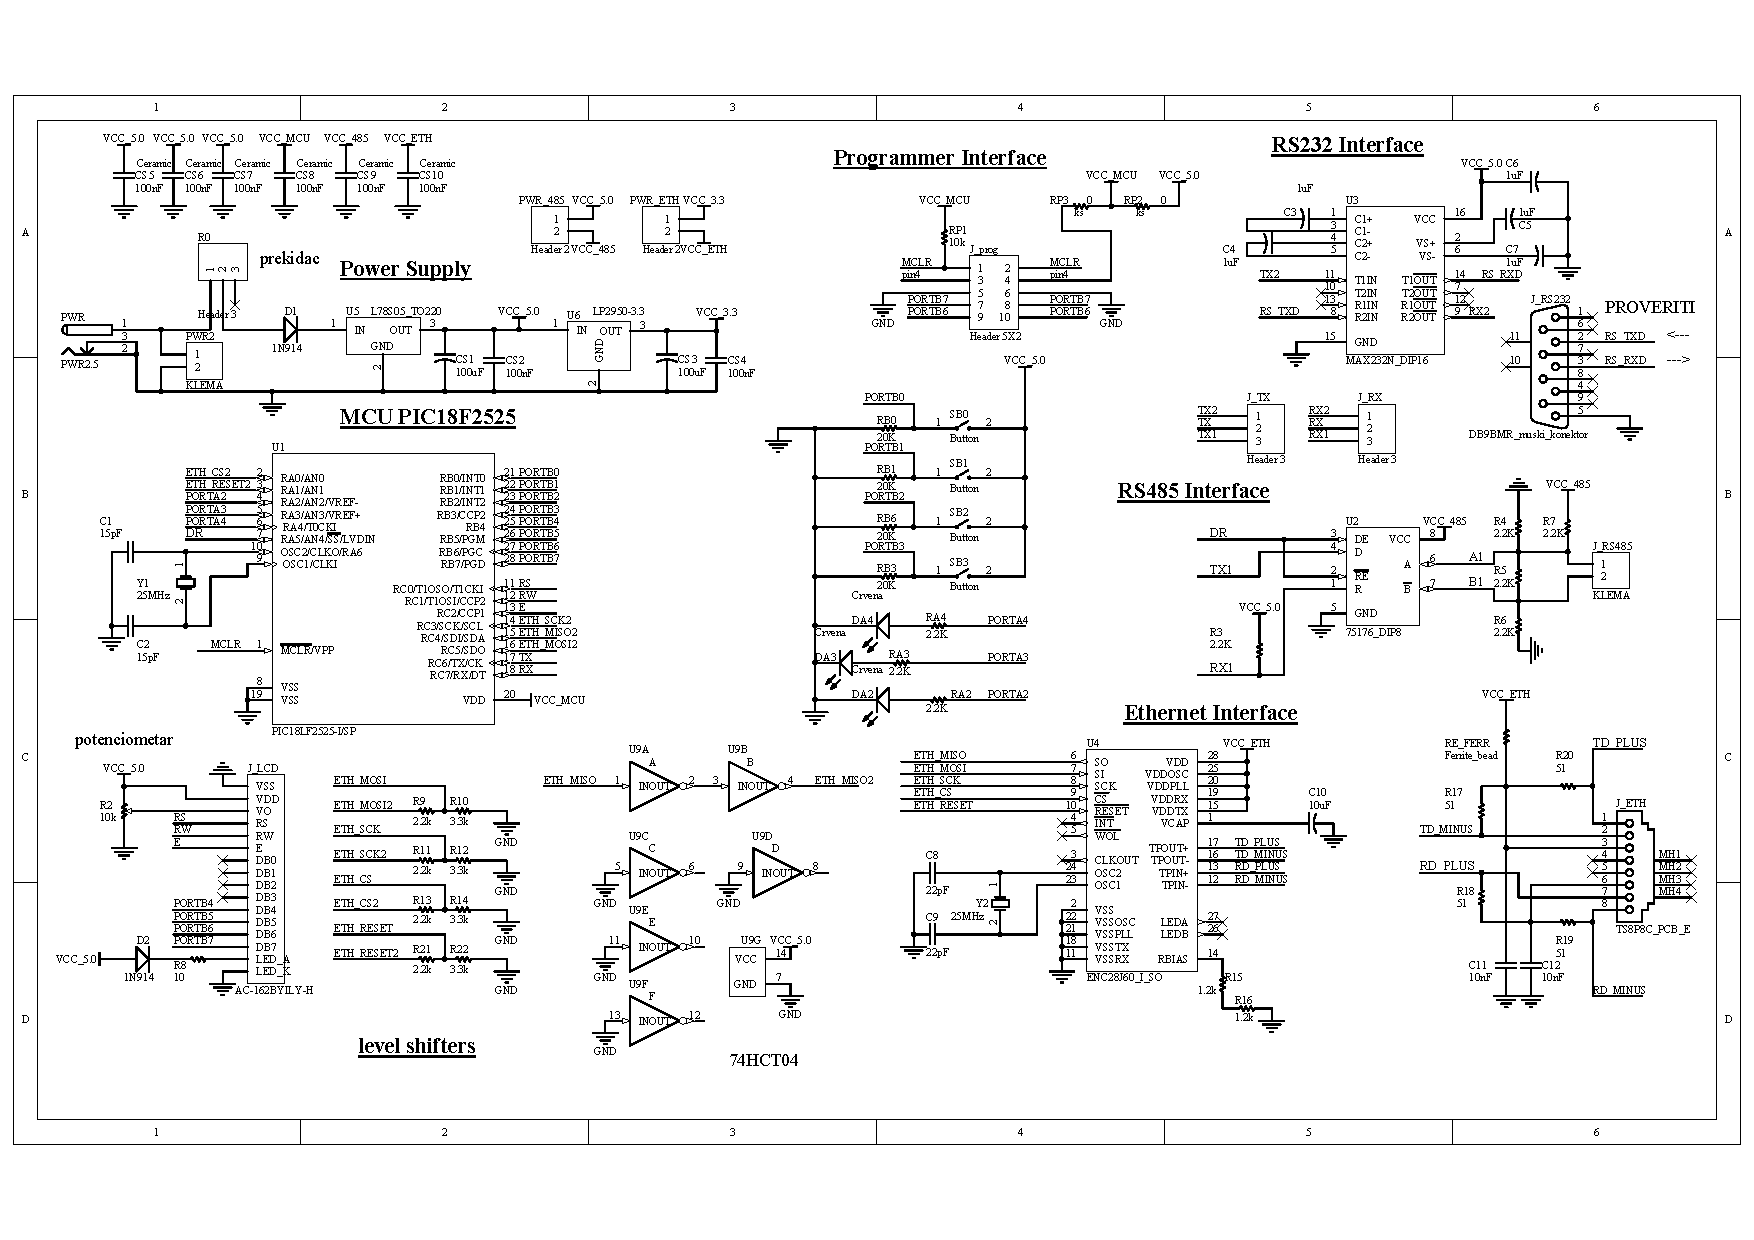
\includegraphics[width=1.2\textwidth]{MasterSema.pdf}
      \caption{Električna šema Master automata}
    \end{figure}
     \begin{figure}[ht]
    \begin{tabular}{|c|c|p{10cm}|}
      \hline
      Port & Smer & Opis \\
      \hline
      PORTA.F5 & Izlaz & DR - Write/read kontrola RS485 drajvera SN65176, Postavlja se na 1 pri upisu. \\
      \hline
      PORTB.F4-F7 & Izlaz & Deo magistrale za prenos podataka između LCD-a i PIC-a \\
      \hline
      PORTC.F0 & Izlaz & RS, Data/Instruction select kontrolni signal LCD displeja \\
      \hline
      PORTC.F1 & Izlaz & Read/Write za LCD, 0 je za čitanje \\
      \hline
      PORTC.F2 & Izlaz & Enable signal za LCD \\
      \hline
      PORTA.F0 & Izlaz & Ethernet reset \\
      \hline
      PORTA.F1 & Izlaz & Ethernet chip select \\
      \hline
      PORTC.F6 & Izlaz & TX za UART \\
      \hline
      PORTC.F7 & Izlaz & RX za UART \\
      \hline
      PORTB.F0 & Ulaz & Inkrement dugme \\
      \hline
      PORTB.F1 & Ulaz & Dekrement dugme \\
      \hline
    \end{tabular}
    \caption{Tabela portova mikrokontrolera}
  \end{figure}


  \begin{figure}[ht]
    \hspace{-1cm}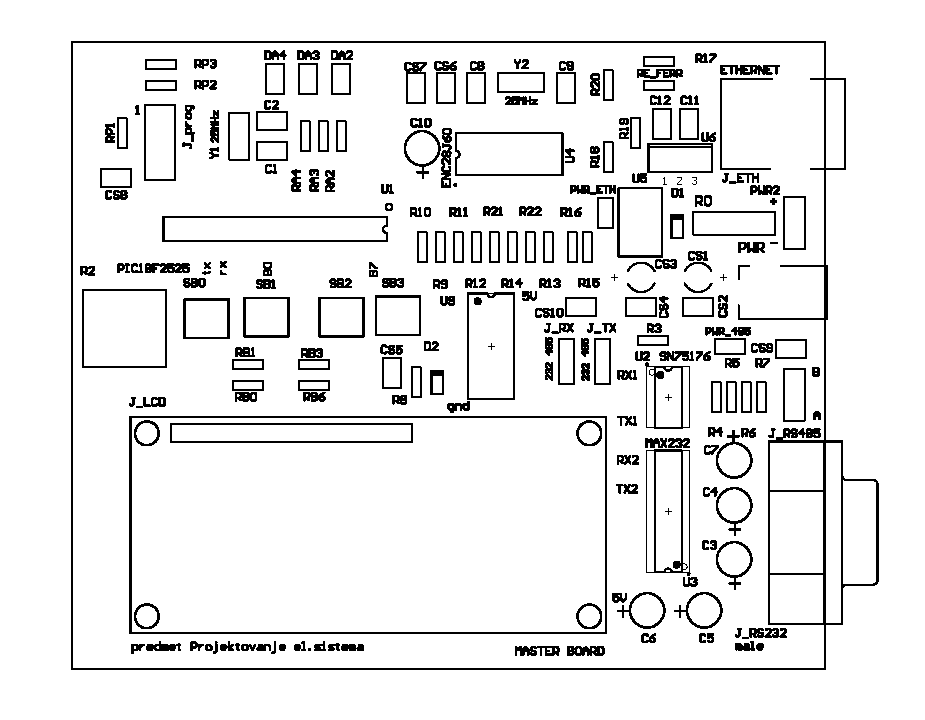
\includegraphics[width=1.1\textwidth]{MasterTopOverlay.pdf}
    \caption{Top overlay Master automata}
  \end{figure}
\clearpage



  \subsection{Prikaz sadržaja displeja Master automata}
  Master automat sadrži 2x16 LCD displej na kome prikazujemo podatke od značaja, naime programe i statuse bašti. 
  Imamo dvadeset različitih prikaza, od kojih su šestnaest za programe a ostala četiri za stanja Slejv automata.
  Prikazi se menjaju pritiskom na jedan od dva tastera, Inkrement i Dekrement, povezani na \texttt{PORTB.F0} i \texttt{PORTB.F1} respektivno.
  

  \begin{figure}[ht]
    \centering
    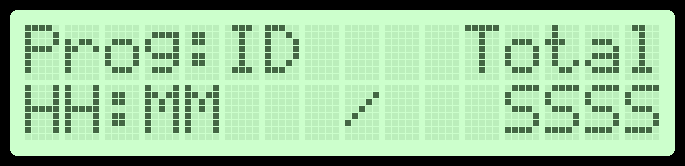
\includegraphics[width=0.48\textwidth]{ProgLCD}
    \caption{Prikaz programa}
  \end{figure}
 \begin{figure}[ht]
    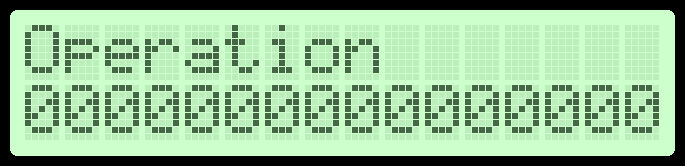
\includegraphics[width=0.48\textwidth]{operation}\hfill
    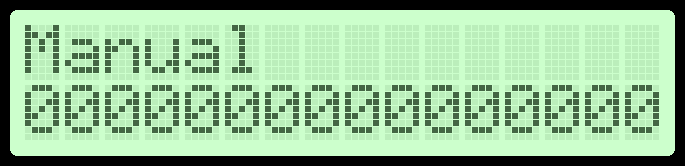
\includegraphics[width=0.48\textwidth]{manual}
    \caption{Prikaz dostupnih bašti i bašti koje se ručno zalivaju}
  \end{figure}
 \begin{figure}[ht]
  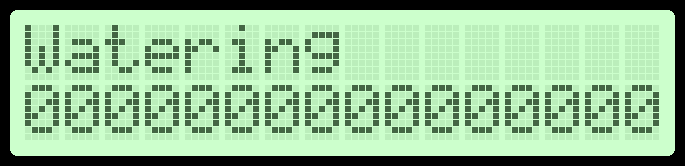
\includegraphics[width=0.48\textwidth]{watering}\hfill
  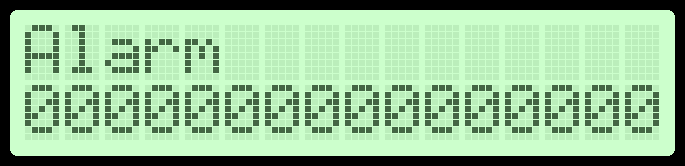
\includegraphics[width=0.48\textwidth]{alarm}
  \caption{Prikaz bašti koje se trenutno zalivaju i čiji je alarm uključen}
 \end{figure}

\clearpage

\subsection{Hardverska realizacija Slejv automata}
  Slejv automat je realizovan na razvojnoj ploči sa mikrokontrolerom PIC16F877A. 
  Mikrokontroler radi na taktu od 20 MHz i napajanju od 5 V, a u okviru sistema koristi digitalne ulaze i izlaze, UART komunikaciju, Tajmer 1, A/D konvertor i 16x2 LCD displej. 
  Slejv je postavljen kod pumpe za zalivanje i zadužen je za lokalno upravljanje pumpom, očitavanje senzora protoka, prikaz stanja na displeju i komunikaciju sa Master automatom.

  Najvažniji elementi Slejv automata su:
  \begin{itemize}
    \item{mikrokontroler PIC16F877A,}
    \item{RS-232/RS485 komunikacioni drajveri,}
    \item{16x2 LCD displej,}
    \item{blok za napajanje razvojne ploče,}
    \item{konektor za programiranje mikrokontrolera,}
    \item{taster za manuelno pokretanje ili zaustavljanje zalivanja,}
    \item{taster za resetovanje lokalnog stanja,}
    \item{analogni ulaz za senzor protoka,}
    \item{LED indikatori za stanje sistema, zalivanje i alarm,}
    \item{prekidači za podešavanje ID broja Slejv automata.}
  \end{itemize}

  Kao i u korišćenim razvojnim sistemima iz vežbi, izbor između RS-232 i RS485 veze vrši se kratkospojnicima na ploči. 
  RS-232 je pogodan za razvoj i testiranje sa jednim uređajem na malom rastojanju, dok se u normalnom radu sistema koristi RS485, jer omogućava povezivanje većeg broja Slejv automata na zajedničku magistralu.

  Raspored korišćenih pinova u realizovanom firmveru prikazan je u tabeli:

  \begin{center}
  \small
  \begin{tabular}{|m{3cm}|m{2cm}|m{8cm}|}
    \hline
    Pin/port & Smer & Namena \\ \hline
    \texttt{PORTB.F0} & ulaz & Taster za manuelno pokretanje i zaustavljanje zalivanja \\ \hline
    \texttt{PORTB.F2} & ulaz & Taster za resetovanje lokalnog stanja Slejva \\ \hline
    \texttt{PORTA.F0} & ulaz & Analogni ulaz A/D konvertora za senzor protoka \\ \hline
    \texttt{PORTA.F2} & izlaz & Indikacija da je sistem uključen \\ \hline
    \texttt{PORTA.F3} & izlaz & Indikacija rada pumpe, odnosno aktivnog zalivanja \\ \hline
    \texttt{PORTA.F4} & izlaz & Indikacija alarma protoka \\ \hline
    \texttt{PORTC.F5} & izlaz & \texttt{DR} signal za izbor smera RS485 drajvera \\ \hline
    \texttt{PORTC.F6} & izlaz & UART TX linija \\ \hline
    \texttt{PORTC.F7} & ulaz & UART RX linija \\ \hline
    \texttt{PORTD.F0-F3} & ulaz & Četvorobitni ID Slejv automata \\ \hline
    \texttt{PORTD.F4-F7} & izlaz & Četvorobitna magistrala podataka LCD displeja \\ \hline
    \texttt{PORTC.F0} & izlaz & \texttt{RS} kontrolni signal LCD displeja \\ \hline
    \texttt{PORTC.F2} & izlaz & \texttt{EN} kontrolni signal LCD displeja \\ \hline
  \end{tabular}
  \end{center}
  \normalsize

  Na LCD displeju Slejv automata prikazuju se podaci potrebni za lokalni nadzor rada pumpe. 
  Prvi red sadrži trenutno vreme i očitanu vrednost protoka, u obliku:
  \[
    \texttt{T HH:MM:SS Fxxx}
  \]
  Drugi red prikazuje da li su aktivni alarm i manuelni režim, vreme početka programa i preostalo vreme zalivanja:
  \[
    \texttt{AM S:HH:MM RMM:SS}
  \]
  Karakter \texttt{A} označava aktivan alarm, a karakter \texttt{M} manuelni režim. 
  Kada odgovarajuće stanje nije aktivno, na tom mestu se prikazuje znak \texttt{/}.


\section{Realizacija firmvera Master automata}
  Firmver Master automata pisan je u C jeziku i kompajliran na mikroC PRO kompajleru za PIC seriju mikrokontrolera.
  Kod za firmver se sastoji od funkcija za inicijalizaciju registara mikrokontrolera, inicijalizaciju globalnih promenljivih, funkcija za komunikaciju izmeđju automata i centralnog računarskog sistema, globalnog timer interrupta, funkcija za izpis na LCD i main funkcije.\newline
  U nastavku su date tabele makroa, pinova, varijabli, struktura i funkcija.
  \begin{figure}[ht]
    \caption{Tabela makroa i pinova}
    \begin{tabular}{|c|c|p{5.5cm}|}
      \hline
      Naziv makroa ili pina & Dodeljena vrednost & Opis \\
      \hline
      SPI\_Ethernet\_HALFDUPLEX & 0 & Komunikacija sa CRS je u punom dupleksu\\
      \hline
      SPI\_Ethernet\_FULLDUPLEX & 1 & Komunikacija sa CRS je u punom dupleksu\\
      \hline
      DR & PORTA.F5 & RS-232 kontrola R/W\\
      \hline
      ButtonInc & PORTB.F0 & Inkrement dugme za promenu prikaza\\
      \hline
      ButtonDec & PORTB.F1 &  Dekrement dugme za promenu prikaza\\
      \hline
    \end{tabular}
\end{figure}
\newline
Struktura Mode opisuje program koji zadajemo putem browsera, sadrži sve potrebne elemente za programiranje pumpe bašte.

\begin{figure}[ht]
  \caption{Struktura Mode}
  \begin{tabular}{|p{5cm}|p{5cm}|p{5cm}|}
    \hline
    Naziv člana & Tip & Opis \\ 
    \hline
    startHour & unsigned char & Sat početka programa \\
    \hline 
    startMinute & unsigned char & Minut početka programa \\
    \hline 
    durationsH & unsigned char & Gornje dve cifre trajanja programa \\
    \hline
    durationsL & unsigned char & Donje dve cifre trajanja programa \\
    \hline
  \end{tabular}
\end{figure}

Struktura Garden sadrži potrebni identifikacioni broj programa, kako bi smo osigurali da svaka bašta može da ima svih 16 postojećih programa.
Kako svaki član koristi isti tip podataka, izbegli smo padding, doprineli smo brzini programa i njegovoj čitljivosti i održavanju. \newline

\begin{figure}[ht]
  \caption{Struktura Garden}
  \begin{tabular}{|p{5cm}|p{5cm}|p{5cm}|}
    \hline
    Naziv člana & Tip & Opis \\ 
    \hline
    modeID & unsigned char & Identifikacioni broj programa dodeljen bašti \\
    \hline 
    gardenSend & unsigned char & Marker za slanje programa određenoj bašti \\
    \hline 
  \end{tabular}
\end{figure}

Data je tabela svih globalnih promenljivih korišćenih u Master firmveru.

\begin{figure}[ht]
    \caption{Tabela globalnih promenljivih}
    \begin{tabular}{|c|c|c|p{5cm}|}
      \hline
      Naziv promenljive & Tip & Početna vrednost & Opis \\
      \hline
      Flag 1 & unsigned char & 0x00 & Flag za 125ms \\
      \hline
      FlagRTC & unsigned char & 0x00 & Flag za slanje RTC podataka \\
      \hline
      FlagPoll & unsigned char & 0x00 & Flag da su svi Slejv atuomati prozvani \\
      \hline
      updateLCDFlag & unsigned char & 0x00 & Flag za osvežavanje LCD-a \\
      \hline
      SLAVE\_ID & unsigned char & 0x00 & Jedinstveni identifikacioni broj svakog Slejv automata \\
      \hline
       ByteID & unsigned char & 0x00 & Jedinstveni identifikacioni broj svakog dolazećeg bajta  \\
      \hline 
       cmd[ ] & unsigned char & 0x00 & Komandni bajt svakog Slejva \\ 
      \hline
       Comm[ ] & unsigned char & 0x00 & Niz slejvova koji su se odazvali\\
      \hline
       Status[ ] & unsigned char & 0x00 & Status bajt koji svaki Slejv šalje Masteru na prozivku \\
      \hline
       no\_ch &  unsigned char  & 0x00 & Brojač karaktera u nizu, može da se koristi i za pozicioniranje na početak niza \\
       \hline
        brojac &  unsigned char  & 0x00 & Brojač za tajmer  5x25ms \\
       \hline
        cntTas &  unsigned char  & 0x00 & Brojač za treperenje tastera \\
       \hline
        cntDisp &  unsigned char  & 0x00 & Brojač za prikaze na LCD-u \\
       \hline
        buffer[250] & unsigned char & 0x00 & Buffer za smeštanje odgovora od Slejvova \\
      \hline
      \end{tabular}
\end{figure}

\clearpage

Ispod imamo tabelu svih funkcija korišćene za realizaciju rada Master automata. Odmah nakon tabele slede i njihova objašnjenja.

\begin{figure}[ht]
  \caption{Tabela funckija}
\begin{centering}
  \begin{tabular}{|p{5cm}|p{2cm}|p{8cm}|}
    \hline
      Naziv funkcije & Tip & Opis \\
    \hline
      init() & void & Podešavanje rada pinova mikrokontrolera, konfigurisanje periferija kontrolera, A/D konvertera, prekida, kola tajmera i inicijalizacija UART-a \\
    \hline
      init\_variables & void & Inicijalizacija početnih vrednosti promenljivih \\
    \hline 
     interrupt() & void & Obrada prekida i debounce tastera\\ 
     \hline
     unsigned int SPI\_Ethernet\_UserTCP(unsigned char *remoteHost, unsigned int remotePort, unisgned int localPort, unsigned int reqLength, char *canCloseTCP) & u\_int & Obrađuju se zahtevi koji pristižu iz WEB pretraživača i izvršava se slanje podataka preko Etherneta \\
     \hline
     formBuffer() & void & Formira Niz podataka koji dobije od Slejva \\ 
     \hline
     appendBuffer() & void & Dodaje članove u niz \\
     \hline
     transmit() & void & Slanje podataka preko UARTA \\
     \hline
     updateLCD() & void & Ispis na LCD ekranu \\ 
     \hline
     lcdDisplayProgram(struct Mode Program, unsigned char ID) & void & Formatiranje prikaza programa \\
     \hline
     lcdDisplayUchar(unsigned char row, unsigned char col, unsigned char value) & void & Formaitranje prikaza unsigned chara \\
     \hline 
     lcdDisplayBit(unsigned char mask) & void & Formatiranje prikaza bitova na ekranu \\
     \hline
     main() & void & Glavna funkcija programa u kojoj se vrši komunikacija i osvežavanje LCD-a \\
     \hline
   \end{tabular}
\end{centering}
\end{figure}


\clearpage
  \subsection{Detaljan opis najvažnijih funkcija sa segmentima koda}
  \textbf{Funkcija init\_variables} služi za inicijalizaciju varijabli na njihovu podrazumevanu početnu vrednost.
  \begin{minted}{C}
  void init_variables() {

  no_ch = 0x00;
  ByteID = 0x00;
  Flag1 = 0x00;
  FlagRTC = 0x00;
  FlagPoll = 0x00;
  updateLCDFlag = 0x00;
  btnCnt = 0x00;
  cntDisp = 0x00;
  hours = 0x00;
  minutes = 0x00;
  seconds = 0x00;
  SLAVE_ID = 0x0F;
  for (i = 0; i < 16; i++) {
    Comm[i] = 0x00;
    Status1[i] = 0x00;
    Program[i].startHour = 0x00;
    Program[i].startMin = 0x00;
    Program[i].durationsH = 0x00;
    Program[i].durationsL = 0x00;
    Garden[i].modeID = 0x00;
    Garden[i].gardenSend = 0x00;
  }
}
\end{minted}
\textbf{Funkcija init} ima zadatak da inicijalizacije portove, registre, UART Baud rate, tajmerski prekid i ethernet.
\begin{minted}{C}
void init() {

  PIR1 = 0b00000000; // flegovi prijema preko UART-a
  PIE1 = 0b00100001; // dozvola prekida za UART, RCIE, TMR1IE
  // PIE1.TMR1IE = 1;
  // PIE1.RC1IE=1;

  T1CON = 0b10110000; // konfiguracija za tajmer1
  T1CON.TMR1ON = 1;
  /*16-bit operation
   preskaler 1:8
   25MH T0=40ns
   40ns*4*8=1.28us
   25ms=25000us=1.28*19531=  B5B3 */
  TMR1L = 0xB5;
  TMR1H = 0xB3;

  INTCON = 0b01000000; // periferijski interapt
  INTCON.GIE = 1;      // globalna dozvola prekida

  // svi pinovi na portu A su izlazi (vidi na semi)
  TRISA = 0x00;
  // obrati paznju, postoje tasteri na portovima RB0 - RB3, to su digitalni
  // ulazi
  TRISB = 0x0F; // ostali pinovi PORTB su izlazi
  TRISC = 0xD0; // 0b11010000; // ovo je OK

  PORTA = 0x00;
  PORTB = 0x00;
  PORTC = 0x00;

  ADCON0 = 0x00; // iskljucujemo A/D konverziju
  ADCON1 = 0x0F; // svi digitalni
  // PORTA.F0=0;

  UART1_Init(UART_BAUD_RATE);

  // konfigurisemo brzinu od 19200 i dodatne bitove za serijski prenos
  TXSTA.TXEN = 1;
  RCSTA.SPEN = 1;
  RCSTA.CREN = 1;
  SPI1_Init_Advanced(_SPI_MASTER_OSC_DIV64, _SPI_DATA_SAMPLE_MIDDLE,
                     _SPI_CLK_IDLE_LOW, _SPI_LOW_2_HIGH);
  SPI_Ethernet_Init(myMacAddr, myIpAddr, SPI_Ethernet_FULLDUPLEX);
  Lcd_Init();
  Lcd_Cmd(_LCD_CLEAR);
  Lcd_Cmd(_LCD_CURSOR_OFF);
  // UpdateLCD();
}
\end{minted}
\textbf{Funkcije appendBuffer i formBuffer} služe za formiranje nizova koji sadrže odgovore Slejv automata koji će kasnije biti prikazani na CRS, na zahtev klijenta.
\begin{minted}{C}
void appendBuffer(char *p_ch) {
  while ((*p_ch) != 0x00) {
    buffer[no_ch] = *p_ch;
    no_ch++;
    p_ch++;
  }
}
void formBuffer() {
  unsigned char i = 0;
  unsigned char txt[4];
  unsigned char StatusByte = 0x00;
  no_ch = 0x00; // pozicioniranje na pocetak niza
  for (i = 0; i < 16; i++) {
    if (Comm[i] == 1) { // samo slejvovi koji su se odazvali
      appendBuffer("Basta:");
      ByteToStr(i, txt);
      appendBuffer(txt); // append broj baste
      appendBuffer(" ");

      StatusByte = Status1[i];
      // prosto testiranje SWAM nibbla koji slave salje na
      // master i ispisavnje statusa na master racunar
      if (!(StatusByte & STATUS_SYSTEM_BIT)) {
        appendBuffer("OFF\n\n");
      } else if (StatusByte & STATUS_WATER_BIT) {
        if (StatusByte & STATUS_MANUAL_BIT) {
          appendBuffer("Watering(Manual_Mode)\n\n");
          if (StatusByte & STATUS_ALARM_BIT) {
            appendBuffer("ALARM ON\n\n");
          }
        } else {
          appendBuffer("Watering(Automatic_Mode)\n\n");
          if (StatusByte & STATUS_ALARM_BIT) {
            appendBuffer("ALARM ON\n\n");
          }
        }
      } else {
        appendBuffer("IDLE\n\n");
      }
      appendBuffer("<br>")
    }
  }
  buffer[no_ch] = 0x00;
  no_ch++; // kraj stringa
}
\end{minted}
\textbf{Funkcija transmit} ima ulogu slanja bajta putem UART veze, poziva se u main funkciji kako bi se ostvarila komunikacija sa Slejv automatom.
\begin{minted}{C}
void transmit(unsigned char DATA8b) {
  TXREG = DATA8b;
  while (!TXSTA.TRMT)
    ;
}
\end{minted}
\clearpage
\textbf{Funkcija interrupt} je jedna od najbitnijih funkcija u celom firmveru.
Služi za obradu prekida, obradu i debouncing tastera za promenu prikaza na LCD displeju, i komunikaciju između Slejv i Master automata, po protokolu koji je opisan u poglavlju 4.1.
Obrada tranzijentnog stanja tastera vrši se u ovoj funkciji po principu brojača koji broji naniže, oba tastera obrađena su na potpuno isti način.
Bitovi registara tajmera takođe dobijaju potrebne vrednosti, naime \texttt{PIE1.TMR1IE}, čija je namena da dozvoli prekid, ne menja vrednost, dok se \texttt{PIR1.TMR1IF} (Timer interrupt flag) stavlja na nizak nivo.
Nakon što je prekid obrađen, registri dobijaju vrednosti \texttt{TMR1H = 0xB3} i \texttt{TMR1L = 0xB5} kako bi smo osigurali da prekid ostane na 25ms.
\begin{minted}{C}
void interrupt() {
  if ((PIE1.TMR1IE == 1) && (PIR1.TMR1IF == 1)) {
    // prekid tajmera 1 -  na svakih 25ms PIE1.TMR1IE = 1;
    PIR1.TMR1IF = 0;
    if (brojac == 0x04) { // na svakih 125ms prozivka slejvova
      brojac = 0x00;
      Flag1 = 0x01;
    } else {
      brojac++;
    }
    // 25ms
    if (btnCnt > 0)
      btnCnt--;
    if ((ButtonInc == 1) && (btnCnt == 0))
    {
      btnCnt = 20; // 20*25=500ms
      updateLCDFlag = 1;
      if (cntDisp >= 20) {
        cntDisp = 0;
      } else {
        cntDisp++;
      }
    }

    if ((ButtonDec == 1) && (btnCnt == 0))
    {
      btnCnt = 20; // 20*25=500ms
      updateLCDFlag = 1;
      if (cntDisp == 0) {
        cntDisp = 20;
      } else {
        cntDisp--;
      }
    }

    TMR1L = 0xB5;
    TMR1H = 0xB3; /// reset tajmera
  }

  if ((PIE1.RCIE) && (PIR1.RCIF)) { // UART RECIEVE FROM SLAVE
    unsigned char ch;
    PIR1.RCIF = 0; // Recieve flag na 0
    ch = RCREG;    // prima se bajt preko UART-a

    switch (ByteID) {
    case BYTE_ID_IDLE:
      break;
    case BYTE_ID_CMD_BYTE:
      if ((ch & CMD_TYPE_MASK) == STATUS_CODE) {
        if ((ch & CMD_ID_MASK) == SLAVE_ID) {
          Comm[SLAVE_ID] = 1;
          ByteID = BYTE_ID_STATUS_BYTE;
        } else {
          ByteID = BYTE_ID_IDLE;
        }
      } else {
        ByteID = BYTE_ID_IDLE;
      }
      break;
    case BYTE_ID_STATUS_BYTE:
      Status1[SLAVE_ID] = ch; // SWAM0000
      ByteID = BYTE_ID_IDLE;
      break;
    default:
      ByteID = BYTE_ID_IDLE;
      break;
    }
  }
}
\end{minted}
\clearpage
\textbf{Funkcija lcdDisplayUchar} je namenska funkcija za prikazivanje unsigned char karaktera na ekran.
Funkcija dobije dvocifren broj koji prostim brojanjem naniže odvaja u zasebne dve cifre (ćelije) za prikaz na koordinatama prosleđenim kao parametri.
\begin{minted}{C}
void lcdDisplayUchar(unsigned char row, unsigned char col,
                     unsigned char value) {
  unsigned char ones;
  unsigned char tens;
  tens = 0x00;
  ones = value;
  while (ones > 9) {
    ones = ones - 10;
    tens++;
  }
  Lcd_Chr(row, col, tens + '0');
  Lcd_Chr(row, col + 1, ones + '0');
}
\end{minted}
\textbf{Funkcija lcdDisplayBit}
Namenska funkcija za prikazivanje bita statusa uzduž drugog reda ekrana.
\begin{minted}{C}
void lcdDisplayBit(unsigned char mask) {
  int i = 0;

  for (i = 0; i <= 15; i++) {
    if ((Status1[i] & mask) == mask) {
      Lcd_Chr(2, 16 - i, '1');
    } else {
      Lcd_Chr(2, 16 - i, '0');
    }
  }
}
\end{minted}
\textbf{Funkcija lcdDisplayProgram} \newline
Obrada prikaza programa obavlja se u ovoj funkciji.
Funkciji se prosleđuje celokupan struct programa kojeg želimo da prikažemo na ekran. 
Funkcija konverzije cifara za prikaz odrađena je u prethodnim namenskim funkcijama, pa je način prikazivanja jasan i koncizan.
\begin{minted}{C}
void lcdDisplayProgram(struct Mode Program, unsigned char ID) {
  // Lcd_Cmd(_LCD_CLEAR);
  Lcd_Out(1, 1, "Prog:");
  lcdDisplayUchar(1, 6, ID);
  Lcd_Out(1, 9, "    ");
  Lcd_Out(1, 13, "Totl"); // prvi red
  //=====drugi red=====
  lcdDisplayUchar(2, 1, Program.startHour);
  Lcd_Chr(2, 3, ':');
  lcdDisplayUchar(2, 4, Program.startMin);
  Lcd_Out(2, 6, "  ");
  Lcd_Chr(2, 8, '/');
  lcdDisplayUchar(2, 9, Program.durationsH);
  lcdDisplayUchar(2, 11, Program.durationsL);
  Lcd_Out(2, 13, "   ");
}
\end{minted}
\textbf{Funkcija updateLCD} \newline
Celokupna obrada svih 20 prikaza obavljena je u ovoj funkciji.
Vrši se provera brojača koji je vezan za taster na ploči, nakon koje se bira jedan od dvadeset mogućih prikaza.
Prvih šestnaest prikazuju program, njegov broj i njegove podatke.
Dok ostali prikazuju statusne bitove Slejv automata u vidu bitskog vektora.
\begin{minted}{C}
void updateLCD() {
  if (cntDisp <= 16) {
    lcdDisplayProgram(Program[cntDisp], cntDisp);
  } else if (cntDisp == 17) { // System
    Lcd_Out(1, 1, "Operation       ");
    lcdDisplayBit(STATUS_SYSTEM_BIT);
  } else if (cntDisp == 18) { // Watering
    Lcd_Out(1, 1, "Watering        ");
    lcdDisplayBit(STATUS_WATER_BIT);
  } else if (cntDisp == 19) { // Alarm
    Lcd_Out(1, 1, "Alarm           ");
    lcdDisplayBit(STATUS_ALARM_BIT);
  } else if (cntDisp == 20) { // Manual
    Lcd_Out(1, 1, "Manual          ");
    lcdDisplayBit(STATUS_MANUAL_BIT);
  }
}
\end{minted}
\textbf{Funkcija main} \newline
Glavna funkcija u kojoj se najpre pozivaju funkcije za inicijalizaciju, nakon kojih sledi glavna beskonačna petlja iz koje se izlazi isključivo po prekidu tajmera, tjst. na svakih 25ms. 
U beskonačnoj petlji vršimo prozivku svih Slejv automata na svakih 125ms, od kojih kada se prozovu svi, prođe dve sekunde. Prolazak kroz sve bašte označava Flag1.
Najpre se šalje broadcast RTC signal (ako je FlagRTC postavljen sa CRS-a), svim Slejv automatima u isto vreme, kako bi se izbeglo kašnjenje i zadržala tačnost sata realnog vremena.
Nakon slanja podešavanja RTC-a, vreme je da se Slejv automati isprogramiraju. Bira se bašta putem browsera kojoj se, kada ona dođe na red, šalju svi potrebni podaci o programu.
Posle prolaska kroz međukomunikaciju, LCD ekran se osvežava i započinjemo novu iteraciju petlje.
\begin{minted}{C}
void main(void) {
  init();
  init_variables();

  while (1) {
    SPI_Ethernet_doPacket();
    if (Flag1 == 0x01) { // 125ms
      Flag1 = 0x00;
      SLAVE_ID++;             // sledeca basta
      if (SLAVE_ID == 0x10) { // svi slejovi pollovani
        SLAVE_ID = 0x00;
        PORTA.F4 = 1;
      } else
        PORTA.F4 = 0;

      if (Garden[SLAVE_ID].gardenSend == 0x01) {
        DR = 1;
        transmit(MODE_CODE | SLAVE_ID); // prvi komandni bajt
        //// BrojBaste.BrojPrograma.Start 1Byte
        transmit(Program[Garden[SLAVE_ID].modeID].startHour);
        transmit(Program[Garden[SLAVE_ID].modeID].startMin);
        transmit(Program[Garden[SLAVE_ID].modeID].durationsH);
        transmit(Program[Garden[SLAVE_ID].modeID].durationsL);
        DR = 0;
        Garden[SLAVE_ID].gardenSend = 0x00;
        ByteID = BYTE_ID_CMD_BYTE;

      } else if (FlagRTC == 0x01) {
        // saljemo RTC signal svim bastama, da bi smo izbegli kasnjenja
        DR = 1;
        transmit(RTC_BROADCAST); // 0x1F
        // transmit(RTC_CODE|SLAVE_ID);
        transmit(hours);
        transmit(minutes);
        transmit(seconds);
        DR = 0;
        FlagRTC = 0x00;
        ByteID = BYTE_ID_CMD_BYTE;

      } else {
        DR = 1;
        transmit(STATUS_CODE | SLAVE_ID); // pitamo za status slejva
        DR = 0;
        ByteID = BYTE_ID_CMD_BYTE; // ocekujemo cmd_byte
      }

    } // od  if (Flag1 == 0x01)

    if (updateLCDFlag == 1) {
      updateLCDFlag = 0;
      updateLCD();
    }
    // od while(1)
  }
}
\end{minted}


\clearpage

\section{Realizacija firmvera Slejv automata}
  Firmver Slejv automata napisan je za mikroC kompajler i kontroler PIC16F877A. 
  Osnovna uloga firmvera je da lokalno upravlja procesom zalivanja i da Master automatu u svakom trenutku može da vrati ažuran status sistema. 
  Zbog toga je program podeljen na inicijalizaciju periferija, obradu prekida, obradu korisničkih ulaza, komunikaciju i glavnu logiku zalivanja.

  \subsection{Definicija pinova i deklaracija promenljivih}
  Na početku programa definisane su simboličke oznake za ulaze i izlaze koji se koriste u kodu. 
  Time se izbegava direktno korišćenje brojeva pinova u ostatku programa i olakšava se povezivanje opisa firmvera sa električnom šemom razvojne ploče.

  \begin{center}
  \small
  \begin{tabular}{|m{3.5cm}|m{3cm}|m{6.5cm}|}
    \hline
    Oznaka u kodu & Pin & Namena \\ \hline
    \texttt{PinTaster} & \texttt{PORTB.F0} & Manuelno pokretanje ili zaustavljanje zalivanja \\ \hline
    \texttt{PinReset} & \texttt{PORTB.F2} & Resetovanje lokalnog stanja automata \\ \hline
    \texttt{PinSystemOn} & \texttt{PORTA.F2} & Izlazna indikacija da je sistem uključen \\ \hline
    \texttt{PinWatering} & \texttt{PORTA.F3} & Izlazna indikacija rada pumpe \\ \hline
    \texttt{PinAlarm} & \texttt{PORTA.F4} & Izlazna indikacija alarma protoka \\ \hline
    \texttt{DR} & \texttt{PORTC.F5} & Upravljanje smerom RS-232 drajvera \\ \hline
  \end{tabular}
  \end{center}
  \normalsize

  \begin{center}
  \small
  \begin{tabular}{|m{3.6cm}|m{3cm}|m{7cm}|}
    \hline
    Promenljiva & Tip & Opis \\ \hline
    \texttt{GARDEN\_ID} & \texttt{unsigned char} & ID broj Slejv automata, očitava se sa \texttt{PORTD.F0-F3} \\ \hline
    \texttt{Hours}, \texttt{Minutes}, \texttt{Seconds} & \texttt{unsigned char} & Trenutno vreme dobijeno dekodovanjem BCD cifara \\ \hline
    \texttt{ProgStartHour}, \texttt{ProgStartMin} & \texttt{unsigned char} & Vreme početka automatskog zalivanja \\ \hline
    \texttt{WateringSec} & \texttt{unsigned int} & Preostalo vreme zalivanja u sekundama \\ \hline
    \texttt{FlowValue} & \texttt{unsigned char} & Trenutno očitana vrednost senzora protoka \\ \hline
    \texttt{FlowMin}, \texttt{FlowMax} & \texttt{unsigned char} & Minimalna i maksimalna dozvoljena vrednost protoka \\ \hline
    \texttt{ManualMode} & \texttt{bit} & Označava da je zalivanje pokrenuto manuelno \\ \hline
    \texttt{CallFlag} & \texttt{bit} & Označava da je stigla prozivka od Master automata \\ \hline
    \texttt{RTCSetupFlag} & \texttt{bit} & Označava da treba prepisati novo vreme u interni sat \\ \hline
    \texttt{ProgramSetupFlag} & \texttt{bit} & Označava da treba prihvatiti novi program zalivanja \\ \hline
    \texttt{UpdateLCDFlag} & \texttt{bit} & Označava periodično osvežavanje LCD displeja i logike zalivanja \\ \hline
    \texttt{m\_bSystemOn}, \texttt{m\_bWatering}, \texttt{m\_bAlarm} & \texttt{bit} & Interna stanja koja se pakuju u statusni bajt \\ \hline
  \end{tabular}
  \end{center}
  \normalsize

  \subsection{Korišćene funkcije}
  \begin{center}
  \small
  \begin{tabular}{|m{3.8cm}|m{3cm}|m{6.8cm}|}
    \hline
    Funkcija & Povratna vrednost & Opis \\ \hline
    \texttt{init()} & \texttt{void} & Podešava smer portova, A/D konvertor, Tajmer 1, UART i prekide \\ \hline
    \texttt{init\_variables()} & \texttt{void} & Postavlja početne vrednosti globalnih promenljivih i čisti LCD \\ \hline
    \texttt{interrupt()} & \texttt{void} & Obrađuje prekid Tajmera 1 i prijem bajtova preko UART-a \\ \hline
    \texttt{ProcessInputs()} & \texttt{void} & Obrađuje tastere za manuelno zalivanje i reset sa debounce zaštitom \\ \hline
    \texttt{IncrementTime()} & \texttt{void} & Uvećava interni sat za jednu sekundu \\ \hline
    \texttt{DecodeTime()} & \texttt{void} & Pretvara BCD cifre sata u promenljive \texttt{Hours}, \texttt{Minutes} i \texttt{Seconds} \\ \hline
    \texttt{ReadADC()} & \texttt{unsigned char} & Pokreće A/D konverziju i vraća vrednost protoka iz registra \texttt{ADRESH} \\ \hline
    \texttt{buildStatusByte()} & \texttt{unsigned char} & Formira statusni bajt koji Slejv šalje Masteru \\ \hline
    \texttt{UpdateLCD()} & \texttt{void} & Ispisuje trenutno vreme, protok, alarme, program i preostalo vreme zalivanja \\ \hline
    \texttt{transmit()} & \texttt{void} & Šalje jedan bajt preko UART predajnika \\ \hline
  \end{tabular}
  \end{center}
  \normalsize

  \subsection{Inicijalizacija}
  Funkcija \texttt{init()} podešava hardver Slejv automata. 
  Port A se delimično koristi za analogni ulaz senzora protoka, a delimično za izlazne indikacije. 
  Port B je podešen kao ulaz za tastere, port C sadrži UART linije, LCD kontrolne linije i \texttt{DR} signal RS-232 drajvera, dok se port D koristi i za ID uređaja i za podatke LCD displeja.

  A/D konvertor je uključen preko registara \texttt{ADCON0} i \texttt{ADCON1}. 
  Rezultat konverzije se koristi kao osmobitna vrednost protoka, tako što se čita registar \texttt{ADRESH}. 
  Tajmer 1 se podešava tako da prekid nastaje na svakih 100 ms. 
  Početne vrednosti \texttt{TMR1H = 0x0B} i \texttt{TMR1L = 0xDC} odgovaraju intervalu od 100 ms za takt mikrokontrolera od 20 MHz i preskaler 1:8. 
  UART se inicijalizuje na 19200 bps, a zatim se dozvoljavaju prekidi Tajmera 1 i prijema preko UART-a.

  \subsection{Obrada prekida}
  Funkcija \texttt{interrupt()} ima dve glavne grane. 
  Prva obrađuje prekid Tajmera 1. 
  Pošto tajmer generiše prekid na svakih 100 ms, brojač \texttt{Counter} se koristi da se posle deset intervala dobije period od jedne sekunde. 
  Tada se pozivaju \texttt{IncrementTime()} i \texttt{DecodeTime()}, a \texttt{UpdateLCDFlag} se postavlja na jedinicu. 
  U svakom tajmerskom prekidu poziva se i \texttt{ProcessInputs()}, čime se tasteri očitavaju dovoljno često da se pouzdano detektuje pritisak.

  Druga grana prekida obrađuje UART prijem. 
  Primljeni bajt se čita iz registra \texttt{RCREG}, a promenljiva \texttt{ByteID} određuje da li se očekuje prvi komandni bajt ili neki od bajtova korisnog sadržaja. 
  Ako prvi bajt odgovara adresi trenutnog Slejva i tipu komande, postavlja se odgovarajući fleg:
  \begin{itemize}
    \item{\texttt{CallFlag} za statusnu prozivku,}
    \item{\texttt{RTCSetupFlag} za podešavanje sata,}
    \item{\texttt{ProgramSetupFlag} za prihvatanje novog programa zalivanja.}
  \end{itemize}
  Na ovaj način se u prekidu radi samo prijem i osnovno dekodovanje poruke, dok se duža obrada prebacuje u glavnu petlju.

  \subsection{Glavna petlja i logika zalivanja}
  Funkcija \texttt{main()} najpre poziva inicijalizacione funkcije za registre, promenljive i LCD, a zatim ulazi u beskonačnu petlju. 
  U petlji se proveravaju flegovi koje su postavili prekidi i korisnički ulazi.

  Reset događaj zaustavlja zalivanje, briše manuelni režim, gasi alarm i vraća sistem u osnovno uključeno stanje. 
  Manuelni taster radi kao prekidač. 
  Kada se manuelni režim uključi, pumpa se pokreće i u simulacionoj verziji programa dobija vreme rada od 180 sekundi. 
  Ponovnim pritiskom tastera zalivanje se zaustavlja.

  Automatsko zalivanje se pokreće kada su ispunjeni sledeći uslovi:
  \[
  \begin{aligned}
    \texttt{m\_bWatering} &= 0,\\
    \texttt{Seconds} &= 0,\\
    \texttt{Hours} &= \texttt{ProgStartHour},\\
    \texttt{Minutes} &= \texttt{ProgStartMin}.
  \end{aligned}
  \]
  Tada se preostalo vreme zalivanja postavlja na trajanje primljeno od Master automata, aktivira se izlaz pumpe i postavlja se status da je zalivanje u toku. 
  Svake sekunde se \texttt{WateringSec} smanjuje za jedan. 
  Kada dostigne nulu, izlaz pumpe se gasi i Slejv prelazi u stanje čekanja sledećeg programa ili manuelne komande.

  \subsection{Nadzor protoka i alarm}
  Vrednost senzora protoka očitava se funkcijom \texttt{ReadADC()}. 
  Alarm se proverava samo dok je zalivanje aktivno. 
  Ako je očitana vrednost manja od \texttt{FlowMin} ili veća od \texttt{FlowMax}, postavljaju se \texttt{PinAlarm} i \texttt{m\_bAlarm}. 
  U suprotnom se alarm gasi. 
  U implementiranoj verziji početne granice su \texttt{FlowMin = 20} i \texttt{FlowMax = 60}. 
  Time se detektuju i kvarovi sa premalim protokom, na primer zapušeno crevo ili prazna posuda, i stanja sa prevelikim protokom, na primer pucanje cevi.

  \subsection{LCD prikaz Slejv automata}
  Funkcija \texttt{UpdateLCD()} osvežava oba reda displeja. 
  Prvi red prikazuje tekuće vreme i trenutnu vrednost protoka. 
  Drugi red prikazuje alarm, manuelni režim, vreme početka programa i preostalo vreme do gašenja pumpe. 
  Preostalo vreme se prikazuje u formatu minuta i sekundi pomoću funkcije \texttt{LcdOutDuration()}.

\newpage
\section{Postupak verifikacije i vrednovanja koda }
 \subsection{Rezultat rada sistema}
  Verifikacija sistema vrši se povezivanjem Master i Slejv razvojne ploče preko RS-232 veze i učitavanjem odgovarajućih firmvera u mikrokontrolere. 
  ID Slejv automata podešava se prekidačima na donja četiri bita porta D. 
  Nakon uključivanja napajanja proverava se da li se na LCD displeju prikazuje trenutno vreme, vrednost protoka, status alarma i preostalo vreme zalivanja.

  Ispravnost komunikacije proverava se periodičnom prozivkom. 
  Master na svakih 125 ms proziva sledeći Slejv i očekuje odgovor sa komandnim i statusnim bajtom. 
  Kada se Slejv odazove, na strani Mastera se ažurira status odgovarajuće bašte, a preko CRS-a se može očitati da li je sistem uključen, da li je zalivanje aktivno, da li postoji alarm i da li je rad pokrenut manuelno.

  Automatski rad proverava se slanjem programa zalivanja sa Master automata. 
  Nakon prijema vremena početka i trajanja zalivanja, Slejv čuva program, prikazuje vreme početka na displeju i čeka poklapanje sa internim satom. 
  Kada se vreme poklopi, uključuje se izlaz pumpe, pali se indikacija zalivanja, a preostalo vreme na displeju počinje da se smanjuje. 
  Po isteku zadatog vremena pumpa se automatski isključuje.

  Manuelni rad proverava se pritiskom tastera na \texttt{PORTB.F0}. 
  Prvi pritisak pokreće zalivanje i postavlja status manuelnog režima, a drugi pritisak zaustavlja zalivanje. 
  Reset taster na \texttt{PORTB.F2} vraća Slejv u početno stanje i gasi alarm i pumpu.

  Alarm protoka proverava se promenom analogne vrednosti na ulazu senzora protoka. 
  Dok pumpa radi, vrednost ispod minimalne ili iznad maksimalne granice aktivira izlaz alarma i statusni bit alarma u odgovoru Slejva. 
  Kada se vrednost vrati u dozvoljeni opseg, alarm se gasi.

  Komunikacija u sistemu proverava se putem centralnog računarskog sistema, gde se na /s zahtev dobijaju povratne informacije o statusu Slejv automata, koji Master automat čuva u svoj buffer.
  Kada se proveri ispravnost rada Slejv automata kako na lokalnom Master LCD-u, tako i na CRS-u, možemo biti sigurni da je sistem operativan.
  \subsection{Stepen ispunjenosti korisničkih zahteva}
  Realizovani Slejv automat ispunjava osnovne zahteve lokalnog uređaja za zalivanje. 
  Uređaj može da prihvati program rada od Master automata, da samostalno pokrene zalivanje u zadato vreme, da isključi pumpu po isteku trajanja programa i da omogući manuelno pokretanje ili zaustavljanje zalivanja. 
  Interni sat može da se podesi daljinski preko Master automata, što omogućava usklađen rad svih Slejv uređaja u sistemu.

  Status sistema dostupan je Master automatu kroz periodični odgovor Slejva. 
  Statusni bajt sadrži informacije o uključenosti sistema, aktivnom zalivanju, alarmu i manuelnom režimu, što odgovara zahtevima za periodično očitavanje stanja bašte. 
  Lokalni LCD prikazuje trenutno vreme, vrednost protoka, vreme početka programa i preostalo vreme zalivanja, pa korisnik na samom uređaju može da proveri trenutno stanje.

  Nadzor protoka je realizovan preko A/D konvertora i poređenja sa minimalnom i maksimalnom dozvoljenom vrednošću. 
  Time je ispunjen zahtev za signalizaciju neispravnog protoka tokom rada pumpe. 
  U trenutnoj verziji firmvera granice protoka su definisane u programu kao početne vrednosti, dok se daljinsko podešavanje granica može dodati proširenjem protokola na isti način kao što je realizovano podešavanje programa zalivanja.

  Realizovani Master automat ispunjava zahteve glavnog kontrolera komunikacije na magistralama Master-Slejv i Master-CRS. 
  CRS komunicira sa Master automatom putem internet browsera koristeći HTTP protokol i GET zahtev, upisivanjem komande direktno u search bar.
  Master automat čuva podatke o svakom zasebnom programu i svakoj bašti ponaosob. 
  Može da programira Slejv automate UART protokolom, preko RS-232 porta za kratke distance, da preko istog protokola prihvata podatke, čuva ih i direktno prikazuje u internet pretraživač u vidu stringa.
  Na svom lokalnom LCD-u prikazuje mogućih 16 programa zalivanja zajedno sa njihovim parametrima, kako i njihove statusne poruke.

\section{Detaljno uputstvo za upotrebu}

  Pre korišćenja Slejv automata potrebno je podesiti njegov ID broj pomoću prekidača povezanih na \texttt{PORTD.F0-F3}. 
  Svaki Slejv u sistemu mora da ima različit ID u opsegu od 0 do 15. 
  Nakon toga se Slejv povezuje sa Master automatom preko RS-232 konektora i uključuje se napajanje razvojne ploče.

  Po uključenju, na LCD displeju Slejva treba da se prikažu trenutno vreme, vrednost protoka i status programa. 
  Ako je potrebno sinhronizovati vreme, sa CRS-a se preko Master automata šalje komanda za podešavanje sata. 
  Master zatim broadcast porukom šalje sat, minut i sekund svim Slejv uređajima.

  Program zalivanja se zadaje preko CRS-a izborom programa i dodelom tog programa odgovarajućoj bašti. 
  Master tada šalje Slejvu vreme početka i trajanje zalivanja. 
  Slejv prihvata program, upisuje ga u aktivne promenljive i na LCD displeju prikazuje zadato vreme početka. 
  Kada interni sat dostigne zadato vreme, zalivanje se pokreće automatski.

  Manuelno zalivanje pokreće se pritiskom tastera na \texttt{PORTB.F0}. 
  Ako zalivanje nije bilo aktivno, pritisak tastera uključuje pumpu i postavlja manuelni režim. 
  Ako je zalivanje već aktivno, sledeći pritisak tastera ga zaustavlja. 
  Reset taster na \texttt{PORTB.F2} koristi se kada je potrebno odmah zaustaviti rad pumpe i vratiti lokalne statuse u početno stanje.

  Tokom zalivanja treba pratiti LCD displej i indikacione diode. 
  Indikacija zalivanja pokazuje da je pumpa uključena, a alarmna indikacija se uključuje ako je protok izvan dozvoljenog opsega. 
  U tom slučaju potrebno je proveriti dovod vode, pumpu, creva i senzor protoka. 
  Kada se protok vrati u dozvoljene granice, alarm se automatski gasi pri sledećem očitavanju senzora.
  
  \clearpage
  \section{Appendix}
  Appendix sadrži sve vrednosti standarda prenosa koje su definisane u deljenom fajlu \texttt{config.h} \newline
  \begin{minted}{C}
    // serijski prijem (UART) ================================
#define UART_BAUD_RATE 19200
// Protokol Master -> Slave:==============================
/*
 * ========================================================
 *RTC promenljive 011|x|idid| -> 0x60 + 3 Bytes HH|MM||SS
 *Biranje moda 101|x|idid| -> 0xA0 + 5 Bytes /pXX|HH|MM|SS|SS
 * ========================================================
 */
#define RTC_CODE 0x60
#define RTC_BYTES 3 // DONE
#define MODE_CODE 0xA0
#define MODE_BYTES 5
#define RTC_BROADCAST 0x7F
// Slave -> Master status response byte.
#define STATUS_CODE 0x20
// Byte-id states used while receiving protocol payload bytes.
// 0 means no payload is currently being received.
#define BYTE_ID_IDLE 0x00
#define BYTE_ID_RTC_HOUR 0x04
#define BYTE_ID_RTC_MIN 0x03
#define BYTE_ID_RTC_SEC 0x02
#define BYTE_ID_MODE_PROGRAM 0x09
#define BYTE_ID_MODE_START_HOUR 0x08
#define BYTE_ID_MODE_START_MIN 0x07
#define BYTE_ID_MODE_DURATION_H 0x06
#define BYTE_ID_MODE_DURATION_L 0x05
#define STATUS_SYSTEM_BIT 0x80 // bit7
#define STATUS_WATER_BIT 0x40  // bit6
#define STATUS_ALARM_BIT 0x20  // bit5
#define STATUS_MANUAL_BIT 0x10 // bit4
// MASKE
#define CMD_TYPE_MASK 0xE0  // Top 3 command bits
#define CMD_ID_MASK 0x0F    // bottom 4 SLAVE ID bits
#define CMD_INOUT_MASK 0x10 // bit4
// ETHERNET
#define MAC_ADDR {0x00, 0x14, 0xA5, 0x76, 0x19, 0x3f}
#define IP_ADDR {10, 99, 12, 1}
#define HTTP_PORT 80
// OBB MasterRecieve
#define BYTE_ID_IDLE 0x00
#define BYTE_ID_CMD_BYTE 0x02
#define BYTE_ID_STATUS_BYTE 0x01

  \end{minted}

\end{document}
